% !TeX program = xelatex
% !BIB program = biber
\documentclass[UTF8,zihao=-4,fontset=fandol,a4paper]{ctexart}
\usepackage[margin=24mm,headheight=16pt,footskip=12mm]{geometry}
\usepackage{fontspec}
\setmainfont{texgyretermes-regular.otf}[BoldFont=texgyretermes-bold.otf,ItalicFont=texgyretermes-italic.otf,BoldItalicFont=texgyretermes-bolditalic.otf]
\setsansfont{texgyreheros-regular.otf}[BoldFont=texgyreheros-bold.otf,ItalicFont=texgyreheros-italic.otf]
\setmonofont{lmmono10-regular.otf}[Scale=0.84,BoldFont=lmmonolt10-bold.otf,ItalicFont=lmmono10-italic.otf,BoldItalicFont=lmmonolt10-boldoblique.otf]
\usepackage{amsmath,amssymb,amsthm,bm}
\usepackage{graphicx,booktabs,tabularx,longtable,array,multirow}
\usepackage{subcaption,float,placeins}
\usepackage{algorithm,algpseudocode}
\usepackage{tikz}
\usetikzlibrary{arrows.meta,positioning,fit,calc}
\usepackage{xcolor,enumitem,fancyhdr,xurl}
\usepackage[backend=biber,style=gb7714-2015,sorting=none,maxbibnames=3,doi=true,url=true]{biblatex}
\addbibresource{references.bib}
\usepackage[unicode,colorlinks=true,linkcolor=black,citecolor=black,urlcolor=blue!45!black,bookmarksnumbered=true]{hyperref}
\hypersetup{pdftitle={执行证据驱动的机器人行为树接地与模型修订},pdfauthor={匿名稿},pdfsubject={五类机器人操作场景的可复现研究}}
\usepackage{listings,titling}
\setlength{\droptitle}{-30pt}
\lstset{basicstyle=\ttfamily\small,columns=fullflexible,keepspaces=true,breaklines=true,frame=single,rulecolor=\color{black!25},backgroundcolor=\color{black!2},numbers=left,numberstyle=\scriptsize\color{black!50},xleftmargin=2em,framexleftmargin=1.5em,showstringspaces=false,tabsize=4}
\linespread{1.13}
\setlength{\parindent}{2em}
\setlength{\parskip}{1pt}
\setlength{\emergencystretch}{2em}
\renewcommand{\topfraction}{0.93}
\renewcommand{\bottomfraction}{0.85}
\renewcommand{\textfraction}{0.07}
\renewcommand{\floatpagefraction}{0.85}
\setcounter{topnumber}{5}
\setcounter{totalnumber}{6}
\makeatletter
\setlength{\@fptop}{0pt}
\setlength{\@fpsep}{16pt}
\setlength{\@fpbot}{0pt plus 1fil}
\makeatother
\setlist{nosep,leftmargin=2em}
\captionsetup{font=small,labelfont=bf,labelsep=quad}
\captionsetup[subfigure]{font=small,labelfont=normalfont}
\floatname{algorithm}{算法}
\renewcommand{\algorithmicrequire}{\textbf{输入：}}
\renewcommand{\algorithmicensure}{\textbf{输出：}}
\newtheorem{proposition}{命题}
\newtheorem{definition}{定义}
\renewcommand{\proofname}{证明}
\newcolumntype{Y}{>{\raggedright\arraybackslash}X}
\newcommand{\C}{\mathcal{C}}
\newcommand{\A}{\mathcal{A}}
\newcommand{\D}{\mathcal{D}}
\newcommand{\Pset}{\mathcal{P}}
\newcommand{\pre}{\operatorname{pre}}
\newcommand{\add}{\operatorname{add}}
\newcommand{\del}{\operatorname{del}}
\newcommand{\code}[1]{\texttt{\detokenize{#1}}}
\graphicspath{{assets/}}
\pagestyle{fancy}
\fancyhf{}
\fancyhead[L]{\small 执行证据驱动的机器人行为树接地与模型修订}
\fancyhead[R]{\small 中文研究稿}
\fancyfoot[C]{\thepage}
\renewcommand{\headrulewidth}{0.3pt}
\ctexset{section={format=\Large\bfseries,beforeskip=1.1ex plus .3ex,afterskip=.6ex},subsection={format=\large\bfseries,beforeskip=.8ex plus .2ex,afterskip=.4ex}}

\title{\heiti 执行证据驱动的机器人行为树接地与模型修订\\[5pt]\large 五类操作场景的可复现研究}
\author{匿名稿\thanks{本文依据截至2026年9月24日的本地实验记录撰写。作者、单位、基金项目及通信信息不在本稿中预设；实验数据均来自仿真，未包含实体机器人试验。}}
\date{}

\begin{document}
\maketitle
\thispagestyle{plain}
\begin{abstract}
行为树规划依赖符号动作模型与底层控制程序之间的有效对应，但语言模型生成的程序能够完成局部目标，并不意味着其全部执行效果与动作模型一致；同样，视觉模型返回二维坐标也不意味着该点可用于机器人控制。针对上述问题，本文以CABTO的行为树接地思想为基础，研究执行证据驱动的动作模型构造、程序验证与效果修订流程。该流程将给定任务集上的符号完备性、受限程序执行中的接口合规性、整个观测谓词集合上的状态转移一致性以及感知可用性分别检验；对已经获得物理执行见证、但存在遗漏效果的动作，由语言模型依据真实前后状态提出受约束补丁，并在保持程序源码不变的条件下重新规划和执行。在五类MuJoCo操作场景中，最终构建了覆盖9个声明目标的43个场景内接地动作实例。工程迭代后冻结的17次任务执行均通过终态验收，113次动作转移均与最终模型匹配；其中两个单臂场景使用视觉粗定位与RGB几何细化、无weld抓持，三个双臂场景仍使用仿真真值定位和显式weld辅助。对31条双臂训练执行见证的配对审计发现，原模型仅有21条满足全状态等式，经10处模型效果修订后全部匹配。独立的统一腕部与全局相机试验完成5次原控制程序兼容性复验，但28次视觉打点诊断中仍存在误认与拒答，尚不能据此宣称双臂视觉闭环成立。结果支持将CABTO作为可检验的分层系统构造框架，同时表明有限样本一致性、人工接口先验与感知可靠性仍限制其自动化程度及泛化结论。
\end{abstract}
\begingroup\small\noindent\textbf{关键词：}行为树接地；动作模型学习；程序生成；执行反馈；多视角感知\par\endgroup

\begin{center}
\large\bfseries Evidence-Driven Behavior Tree Grounding and Action Model Refinement for Robotic Manipulation
\end{center}
\begingroup\small
\noindent\textbf{Abstract:} Building on CABTO, this paper studies evidence-driven behavior tree grounding with separate checks for task-set completeness, program validity, observable-state transition agreement, and perception usability. Language models propose constrained effect patches from actual execution witnesses; control source code remains unchanged for revalidation. Five MuJoCo scenes contain nine declared goals and 43 grounded actions. Following engineering iterations, all 17 frozen executions and 113 action transitions pass their respective checks. The single-arm scenes use visual localization and no weld assistance; dual-arm scenes retain oracle geometry and explicit welds. A paired audit of 31 dual-arm training witnesses exposes ten models with omitted effects, which are corrected before subsequent task execution. Unified wrist/global cameras preserve control compatibility, but 28 pointing diagnostics still reveal errors and abstentions. The results support a testable construction workflow, not fully autonomous grounding or universal physical consistency.

\noindent\textbf{Key words:} behavior tree grounding; neuro-symbolic robotics; action model learning; code generation; execution feedback; multi-view perception
\endgroup

\section{引言}
机器人操作系统需要同时解决任务层的离散决策与运动层的连续控制。行为树通过条件节点、动作节点及控制流节点组织机器人行为，能够清晰表达执行顺序与状态依赖，也便于在任务执行期间根据当前观测选择动作。然而，行为树结构的可规划性依赖于节点语义已经正确建立：规划器使用的前提与效果必须能够由实际程序及其所调用的控制接口实现。如果这一对应关系仅由人工假定，或者仅依据语言模型对执行结果的自述建立，则符号计划的正确性并不能直接转化为机器人任务的可靠完成。

这一问题至少包含三个尚需区分的子问题。首先，动作库能否覆盖给定目标集合，是关于符号模型的完备性问题；程序能否在满足前提的连续状态下执行，则是另一层问题。其次，即使程序达成了声明的正向效果，也可能遗漏释放、撤离等必要控制步骤，或者引起模型没有记录的状态变化。最后，感知接口中“识别到物体”“得到像素点”和“获得可执行位姿”并不等价。尤其在双臂操作中，夹爪自遮挡、同类物体混淆、容器沿与底面的高度差异，会使语义上看似合理的点偏离真正的接触区或支撑面。将这些问题都归结为语言模型推理不足，容易导致错误修订动作模型，或者以更强控制先验掩盖感知失败。

本文从五类机器人操作场景的连续工程实验出发，对行为树接地过程进行重新组织。核心思路是让语言模型提出候选，而由独立运行时提供可检查的执行见证。我们采用显式细粒度接口生成动作程序，将完整观测状态与符号预测相比较，并把真实遗漏效果反馈给模型。模型修订之后，控制源码保持不变，规划器重新验证声明任务集合，新执行回合重新验证物理效果。感知部分则区分已经进入控制的单臂视觉定位和尚未进入控制的双臂多视角诊断，避免把新的相机图像或二维点输出追记为已有成功任务的感知依据。

本文贡献集中在三个方面，而非提出一个新的大模型或宣称替代运动规划。其一，给出兼容CABTO思想的分层验证表述，明确任务集完备性、全观测状态一致性与普遍物理可执行性之间的边界。其二，构建执行见证约束下的模型效果修订与程序来源追溯流程，在不改写控制源码的条件下检查跨层修订是否真正解释了状态变化。其三，在厨房配对放置、积木堆叠、端盆接球、空中交接和双臂装箱上架五个冻结场景中提供可复查的执行记录、失败案例和统一相机诊断。该研究定位为方法扩展与系统实证分析；现有结果不构成从空动作库到纯视觉双臂控制的完全自主解决方案，也不构成优于其他方法的等预算比较。

\section{相关工作与研究定位}
\subsection{行为树规划与接地}
行为树的模块化控制语义及其状态空间分析已经形成较为系统的研究基础\cite{btbook2018}。BT Expansion在给定动作模型条件下，通过展开前提构造行为树，并讨论符号规划的可靠性与完备性\cite{btexp2021}。这类保证建立在模型与执行节点正确对应的假设之上，不应被解释为对任意生成控制程序或任意连续初态的保证。

CABTO进一步将研究对象从行为树结构扩展到行为树系统本身，联合考虑高层动作模型提出、低层策略采样及跨层修订\cite{cabto2026}。其重要性在于把“节点如何获得物理含义”从隐含前提变成显式问题。本文沿用这一问题划分，但不重复原论文的复杂性结论，也不重新声称行为树接地的原创定义。与原始流程相比，本文重点加强整个观测状态上的经验检验，并对“有限策略采样失败”与“动作模型不一致”采取更保守的区分。对原论文的讨论以用户提供的九页预印本中的定义和算法为依据，文献元数据采用正式出版版本。

\subsection{动作模型学习与任务运动规划}
STRIPS以前提、增加效果和删除效果表示动作，未被效果修改的命题默认保持不变\cite{strips1971}。任务与运动规划进一步耦合离散搜索与连续几何可行性，揭示了抓取方式、物体姿态和后续可达性之间的关联\cite{tamp2021}。从轨迹中学习符号算子的工作将符号状态看作连续状态的有损抽象，说明抽象层面的可达关系并不能保留全部几何信息\cite{silver2021}。

本文的效果修订比一般的动作模型学习更受限制：谓词词表、操作签名和部分前提由工程参考指定，补丁只能解释已有执行见证中的遗漏增删效果，不能借此推断未观测状态中的可执行性。这样的限制降低了当前系统的自动化程度，但也使每次模型变化具有明确的实验依据，并暴露了后续前提学习需要解决的问题。

\subsection{语言模型程序与视觉操作表示}
SayCan将语言层面的任务相关性与已有技能的可执行性结合，为语言指令提供机器人能力约束\cite{saycan2023}。Code as Policies利用语言模型编写程序，组合感知接口与控制原语\cite{cap2023}。VoxPoser通过组合三维价值图组织几何约束\cite{voxposer2023}；ReKep则把操作任务表示为关系关键点约束，并通过优化求解动作\cite{rekep2025}。这些工作表明，中间表示和感知接口的设计会直接影响语言模型知识能否落地。

本文采用程序化中间表示，但并未复现上述方法的训练、基线或优化器。区别在于，我们将程序接口副作用、实际观测状态变化以及源码来源作为独立检查对象。程序能够调用某个名称正确的函数，并不意味着它执行了模型所需的物理步骤；因此，整套抓放隐藏在一个接口中的实现，不能用于证明细粒度程序生成已经成立。

\subsection{多视角与主动感知}
主动感知强调通过观测行为改善任务相关信息，而不仅是增加静态传感器数量\cite{active2018}。Qwen2.5-VL提供了用于语义理解与视觉定位的模型基础\cite{qwen25vl}，但其输出坐标是否能转换为机器人控制目标仍取决于标定、目标身份与接触几何。本文的统一腕部和全局相机只完成安装、动态标定和同状态视角诊断，尚未实现以不确定性驱动的主动选视或基于新相机输出的双臂闭环控制。相机数量增加本身不作为感知改进的充分证据。

\section{问题定义与可验证性质}
\subsection{连续状态、观测抽象与动作程序}
设物理状态为 $x\in\mathcal{X}$，包括机器人关节、物体位姿及相关动态量。接触历史和交接先后关系需要运行时监测记忆 $m\in\mathcal{M}$。因此，以 $z=(x,m)$ 表示完整执行状态，以避免把具有历史依赖的事件谓词误写成仅由当前位姿决定的无记忆变量。监测记忆由可信运行时依据实际事件更新，生成程序不能直接写入成功标志或监测结论。

给定固定谓词词表 $\C$，独立观测映射为
\begin{equation}
    s=\alpha(z)\subseteq\C.
\end{equation}
程序所读取的视觉或几何观测记为 $o=\beta(z)$。$\alpha$与$\beta$的用途不同：$\alpha$提供评估所需的符号事实，$\beta$为控制提供目标信息。仿真真值可以在评估器中使用，但若进入$\beta$或运动反馈，就必须计入控制先验，而不能继续称为纯视觉系统。

一个接地动作实例表示为 $a=(h_a,\pi_a)$，其中 $h_a=(\pre_a,\add_a,\del_a)$ 是符号模型，$\pi_a$是调用许可接口集合$\mathcal{U}$的有限程序。对于满足$\pre_a\subseteq s$的状态，预测后继为
\begin{equation}
    \widehat{s}^{+}=h_a(s)=(s\cup\add_a)\setminus\del_a.
    \label{eq:strips}
\end{equation}
本文实现沿用所用规划内核的规范化约束 $\pre_a\cap\add_a=\varnothing$ 及 $\add_a\cap\del_a=\varnothing$；前提与删除效果可以相交。该规范化不应被理解为所有规划表示的普遍要求。

\subsection{给定任务集上的符号完备性}
给定声明任务集合 $\Pset=\{p_i=(s_i^0,g_i)\}_{i=1}^{N_P}$，候选动作库为$\A$。本文检验的任务集完备性是
\begin{equation}
    \forall p_i\in\Pset,\quad
    \operatorname{BTPlan}(\A,s_i^0,g_i)\text{返回可达目标的符号行为树}.
    \label{eq:complete}
\end{equation}
这里的“完备”描述动作库相对于给定任务集合的覆盖能力，并非声称实现了对任意新任务的求解。它也不同于规划算法自身的完备性。本文采用已有BT Expansion内核验证式\eqref{eq:complete}，不将预先设定的目标顺序直接当作行为树规划结果。

\subsection{全观测状态一致性与经验范围}
执行程序后得到轨迹 $\tau$ 与实际后继状态 $s^{+}=\alpha(z^{+})$。声明效果检查可写为
\begin{equation}
\begin{split}
    G_{\rm dec}={}&[\pre_a\subseteq s]\land[\add_a\subseteq s^{+}]\\
    &\land[\del_a\cap s^{+}=\varnothing]
    \land[(\pre_a\setminus\del_a)\subseteq s^{+}].
\end{split}
\end{equation}
这一检查包含删除效果，但仍未覆盖不在前提中的所有应保持事实。因此，本文进一步要求
\begin{equation}
    G_{\rm full}(s,a,s^{+})=[s^{+}=h_a(s)].
    \label{eq:full}
\end{equation}
“全观测”指固定$\C$中的全部谓词，而不是连续状态$z$的所有分量。没有被词表表达的擦碰、姿态差异或时间属性仍需单独监测。总验收条件还包含接口执行合法性$G_{\rm api}$、有效前态$G_{\rm pre}$以及任务特定物理约束$G_{\rm phy}(\tau)$：
\begin{equation}
    G=G_{\rm api}\land G_{\rm pre}\land G_{\rm full}\land G_{\rm phy}.
    \label{eq:gate}
\end{equation}

\begin{proposition}[声明效果通过不蕴含全状态一致]
存在满足$G_{\rm dec}$的执行见证，但不满足式\eqref{eq:full}。
\end{proposition}
\begin{proof}
取$s=\{p,q\}$，$\pre=\{p\}$，$\add=\{r\}$，$\del=\{p\}$。符号预测为$\{q,r\}$。若实际后继为$\{r\}$，则前提有效，增加与删除效果均满足，保留前提集合为空，故声明效果检查通过；但未声明的$q$丢失，因此全状态等式不成立。
\end{proof}

对于有限执行数据集$\D_a$，定义经验一致性
\begin{equation}
    \operatorname{Consistent}_{\D_a}(a)
    \iff \forall(s,\tau,s^{+})\in\D_a,\ G(s,a,\tau,s^{+})=1.
\end{equation}
该性质不能外推为
$\forall z:\pre_a\subseteq\alpha(z)\Rightarrow\alpha(\operatorname{Exec}(\pi_a,z))=h_a(\alpha(z))$。
两个连续状态可能具有同一符号抽象，却分别对应可达与不可达抓取姿态。有限见证未覆盖的连续变量不能由经验一致性自动消除。类似地，给定采样预算内未找到程序，仅能说明当前搜索失败，不能据此证明相应动作不存在可行实现。

\section{执行证据驱动的接地流程}
\subsection{总体结构与信息边界}
图\ref{fig:framework}给出本研究采用的系统结构。初始输入包括任务集合、谓词语义、许可接口与冻结场景配置。语言模型提出动作模型或程序，规划器与独立运行时分别提供符号和物理反馈。感知模块、控制模块与评估模块的来源分别记录，而不以一个“模型后端”名称概括整个系统。

\begin{figure}[htbp]
\centering
\begin{tikzpicture}[font=\small,box/.style={draw=black!55,rounded corners=2pt,align=center,minimum width=43mm,minimum height=16mm,fill=black!3},arr/.style={-{Latex[length=2mm]},thick}]
\node[box] (task) {任务集与许可接口\\冻结配置、谓词语义};
\node[box,right=9mm of task] (model) {模型提出／参考初始化\\符号完备性检查};
\node[box,right=9mm of model] (code) {受限程序采样\\局部反馈、源码追溯};
\node[box,below=15mm of code] (execute) {实际控制执行\\轨迹、接触、前后状态};
\node[box,left=9mm of execute] (check) {独立验收器\\全状态等式＋物理约束};
\node[box,left=9mm of check] (patch) {证据约束的效果修订\\程序不变、重规划重验};
\draw[arr] (task)--(model);\draw[arr] (model)--(code);\draw[arr] (code)--(execute);\draw[arr] (execute)--(check);\draw[arr] (check)--(patch);\draw[arr] (patch.north)--(task.south);
\draw[arr,dashed] (check.north) -- node[right,font=\scriptsize]{通过后登记} (model.south);
\end{tikzpicture}
\caption{执行证据驱动的行为树接地流程。图中箭头表示本研究实现的信息依赖，不表示各模块已经由一个无需人工干预的代理自主编排。感知诊断与物理验收分别记录，程序返回值不作为成功依据。}
\label{fig:framework}
\end{figure}

本文采用两种初始化方式。Cover从语言模型实际返回的三类动作schema开始，在预定义词表与签名约束下机械替换对象参数，得到七个接地动作；Blocks复用这些schema及兼容程序原文，再独立验证新对象绑定。三个双臂场景采用参考模型初始化：初始模型由工程参考提供，模型进一步根据实际执行中的遗漏效果进行修订。两种方式的自动化程度不同，实验中分别报告，不将参考初始化改称空库学习。

\subsection{局部动作程序的生成与检查}
程序采样提示包括当前动作的终止条件、对象角色、实际可用API以及最近一次失败源码和反馈。不把完整场景任务直接作为每个动作的生成指令，避免模型在Pick动作中继续执行Place甚至回HOME。生成源码经过有限抽象语法树解释器执行；控制接口按动作类型限定，并在任何运动发生前检查调用名称和签名。坐标参数要求来自允许的只读目标接口，不允许直接把日志中的数值抄作未感知的固定目标。

这一限制是项目内的执行约束，而不是对通用Python程序的安全性证明。当前数据来源检查只覆盖实现支持的有限语法子集，也不能阻止错误目标身份或所有不合理几何运算。必要时，运行时进一步检查目标绑定、动作阶段、闭爪与附着的先后关系。接口检查失败的候选保留原始回答和错误信息；不会在后台删除分支、补入缺失动作或修改返回值来使其通过。

图\ref{fig:code}给出实际接受的抓取源码示例。接近、下降、闭爪和抬升由程序显式发出。工程提供的控制器负责轨迹插值、逆运动学与伺服，因而这里的“程序生成”不是学习关节级控制律。在双臂接口中，还分别暴露闭爪与接触门控附着、张爪与解除附着、释放与撤离。对于空臂HOME、同步刚体平移等控制原语，仍保留内部轨迹控制，但不将整套抓放藏入一次夹爪操作。

\begin{figure}[htbp]
\lstinputlisting[language=Python]{assets/generated_pick.py}
\caption{Cover中实际接受的本地模型抓取程序原文。注释与函数内容不做语义改写。程序不直接设置\code{holding}谓词，其效果由可信运行时根据物理状态独立判定。}
\label{fig:code}
\end{figure}

采样Place等动作时，前态通过已接受程序真实执行而建立，不通过写入物体位姿制造持物状态。候选失败后重新初始化同一试验配置，并重放已接受的前置程序，以避免失败动作改变环境后继续比较不等价前态。该过程会产生额外计算与人工调试成本，本文不将其隐含到最终成功次数中。

\subsection{遗漏效果的跨层修订}
若物理程序完成声明目标且满足任务安全条件，但全状态检查不通过，则定义
\begin{equation}
    \Delta^{+}=s^{+}\setminus\widehat{s}^{+},\qquad
    \Delta^{-}=\widehat{s}^{+}\setminus s^{+}.
    \label{eq:delta}
\end{equation}
$\Delta^{+}$表示实际新增而未预测的事实，$\Delta^{-}$表示预测保持或增加、实际却不存在的事实。语言模型接收动作模型、真实前后状态和式\eqref{eq:delta}，输出候选补丁$U^{+},U^{-}$。运行时要求
\begin{equation}
    U^{+}\subseteq\Delta^{+},\quad U^{-}\subseteq\Delta^{-},\quad
    \add'_a=\add_a\cup U^{+},\quad\del'_a=\del_a\cup U^{-}.
    \label{eq:patch}
\end{equation}
同时检查规范化约束、完整见证等式和式\eqref{eq:complete}。不在见证差异中的新谓词、不解释全部差异的补丁或破坏任务可达性的补丁均被拒绝。本阶段保持$\pre_a$与$\pi_a$不变，并为修改后的模型重新登记待验状态，而不是沿用修改前的接受标记。

式\eqref{eq:patch}是一种受限制的效果扩展，不覆盖需要撤销旧效果、引入条件效果或改变谓词定义的情形。例如，若某事实被模型删除但实际保留，直接将其同时加入add可能违反$\add\cap\del=\varnothing$；此时不能强行套用补丁，应保留未解决状态并进入更广泛的模型诊断。对于本研究观察到的十处差异，受约束补丁已经能够解释见证。该结论不代表此类补丁对任意模型错误都足够。

\begin{algorithm}[htbp]
\caption{执行见证约束的模型效果修订与复验}
\label{alg:refine}
\begin{algorithmic}[1]
\Require 任务集$\Pset$；固定观测词表$\C$；候选模型$H$；许可接口$\mathcal{U}$；采样预算$B$
\Ensure 已验证动作库及其证据，或明确的未解决原因
\State 使用符号规划检查$H$对$\Pset$的覆盖，保留提出来源
\For{待验证动作$h_a$}
  \State 通过真实执行已接受程序建立合法前态
  \For{$b=1,\ldots,B$}
    \State 生成或按已记录来源复用程序$\pi_a$，检查语法、接口与坐标来源
    \State 执行$\pi_a$并保存$(s,\tau,s^{+})$；独立检查声明效果和物理约束
    \If{程序异常、声明效果失败或物理约束不满足}
      \State 将失败回传程序采样；不直接判定动作模型不可实现
    \ElsIf{$s^{+}\ne h_a(s)$}
      \State 计算$\Delta^{+},\Delta^{-}$，由模型提出受约束效果补丁
      \State 检查补丁合法性、见证等式与修改后任务集完备性
      \If{补丁通过上述检查}
        \State 更新$h_a\leftarrow h'_a$，保持$\pi_a$源码不变，重新规划并执行
        \State 仅在新回合满足式\eqref{eq:gate}时登记，否则保留为待修订
      \EndIf
    \Else
      \State 登记$(h_a,\pi_a)$及其有限执行见证，结束该动作采样
    \EndIf
  \EndFor
\EndFor
\State 在冻结模型与程序上执行完整任务及稳定窗口验收
\State 若仍有未通过项，则输出具体未解决项而非补写成功状态
\end{algorithmic}
\end{algorithm}

算法\ref{alg:refine}总结了实验中实际采用的验证逻辑。其关键区别不是让模型对自己评分，而是让模型提出可被运行时反驳的修改。应注意，给定确定的前后状态差异，最小效果补丁也可能由规则方法构造；当前结果验证了这一接口的可工作性，尚未证明语言模型相对于确定性差分修订器的必要性或优势。

\subsection{程序复用与证据追溯}
程序复用分为schema级直接复用和提示示例迁移。前者保持源码与哈希不变，仅通过只读角色接口重新绑定对象；后者将旧模型源码作为上下文，再调用模型生成新的程序。两者都需要新场景中的物理验收，但只有后者计作新的生成调用。本文记录原始提示、模型回复、格式提取、执行源码、API调用轨迹、配置哈希与源文件快照，以检查“声称生成的程序”是否就是“实际执行的程序”。

哈希一致性能够检查文件是否变化，却不能证明程序语义正确或数据无偏。因此，本研究把来源追溯与物理验收并列使用，而不把日志齐全视作算法有效性的替代证据。此前参考回放、会话直接编写候选与本地模型实际输出分别保留，最终结果表只纳入指定冻结目录中的执行记录。

\subsection{感知接地与统一相机诊断}
在Cover与Blocks中，视觉语言模型首先提供目标的二维粗点，RGB连通域及几何拟合进一步估计中心。相机标定与显式高度先验将像素映射到三维空间。采用MuJoCo相机坐标约定时，光轴为$-Z$，像素$v$向下；对于相机位置$\bm c$、旋转$R$和内参$(f_x,f_y,c_x,c_y)$，射线可写为
\begin{equation}
\bm d\propto R\begin{bmatrix}(u-c_x)/f_x&-(v-c_y)/f_y&-1\end{bmatrix}^{\!\top},\qquad
\bm p=\bm c+\frac{z_0-c_z}{d_z}\bm d.
\label{eq:ray}
\end{equation}
平面高度$z_0$必须对应被检测的几何特征。若检测碗沿却采用碗底平面，则即使像素接近正确轮廓中心，也会产生系统性水平误差。缓存仅用于任务中位置保持受独立约束的支撑物；缓存读取不重复计作模型调用。

五场景统一相机配置为每只Panda手部一台固定局部外参相机，加一台按桌面坐标规则安装的全局俯视相机，并保留原全景相机。腕部相机位于手部局部$[0,-0.100,0.025]$\,m，固定看向局部$[0,0,0.160]$\,m，垂直视场角$75^\circ$；全局相机位于桌面中心沿世界$X$偏移0.080\,m、桌面上方1.20\,m，视场角$60^\circ$。图像均为$720\times720$。相机随真实父body运动，不根据目标真值跟踪，也不是裁剪全景形成的伪腕部视图。此部分仅增加理想光学节点，尚未建模相机外壳、支架质量与电缆。

\section{实验设计}
\subsection{平台、任务与冻结配置}
实验在MuJoCo仿真器\cite{mujoco2012}中完成，使用Panda单臂或双臂控制底座。环境为MuJoCo~3.10.0、Python~3.11.9、MLX-VLM~0.6.3、MLX~0.31.2、Transformers~5.12.1、OpenCV~4.13.0.92。本地生成主要使用四比特Qwen3.5-9B\cite{qwen35}，视觉粗点主要使用四比特Qwen2.5-VL-3B。前期0.8B、3B和9B的不同提示及解码配置均作为工程诊断，不作为受控的模型规模消融。具体模型标识与数据路径见附录。

表\ref{tab:tasks}说明任务定义。Cover的名称沿用工程目录，但实际任务是厨房三物体配对放置，不是加盖。Handover的三盒画面包含一只活动盒与两只陈列盒，不能理解为连续交接三只盒。Pour以刚性球体表示被转移内容物，不对流体倾倒建模。各场景的机器人基座、桌面、物体几何及控制参数在本次冻结验证中不变；此前为建立可完成基线的工程设计属于先验投入，不归因于模型自动学习。

\begin{table}[htbp]
\centering\small
\caption{五类场景与声明任务。动作数为各场景内接地实例数，不能解释为43种独立学得的技能。}
\label{tab:tasks}
\begin{tabularx}{\linewidth}{l c c Y}
\toprule
场景 & 目标数 & 动作数 & 任务语义与必要终态 \\
\midrule
Cover & 3 & 7 & C1：虾入碗；C2：加苹果上砧板；C3：再加土豆入锅。均释放、撤离并回HOME。\\
Blocks & 3 & 5 & B1：黄块叠绿块；B2：红块叠蓝块；B3：两组堆叠。支撑块保持稳定，末端释放并回HOME。\\
Pour & 1 & 10 & 一臂持源杯、另一臂端盆，球体经倾倒进入盆；分离、源杯回正、容器归位和双臂复位。\\
Handover & 1 & 7 & 无把手茶盒空中交接；接收持有验证先于供方释放，最终桌面支撑并双臂复位。\\
Storage & 1 & 14 & 两件积木进入自由纸箱，双臂抓侧柄抬箱上架；物品保持包含、纸箱获支撑、释放并退手。\\
\bottomrule
\end{tabularx}
\end{table}

\begin{figure}[htbp]
\centering
\begin{subfigure}{.31\linewidth}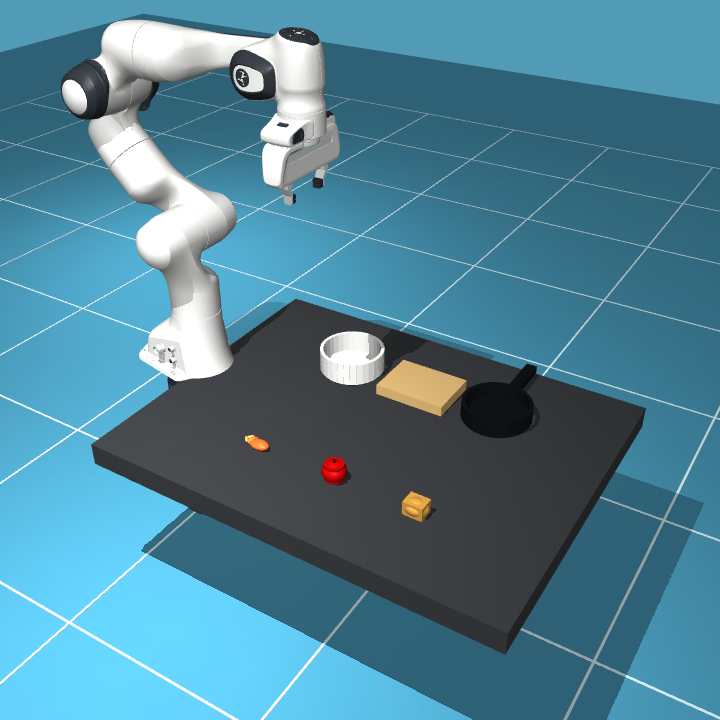
\includegraphics[width=\linewidth]{cover_initial.png}\caption{Cover：厨房配对放置}\end{subfigure}\hfill
\begin{subfigure}{.31\linewidth}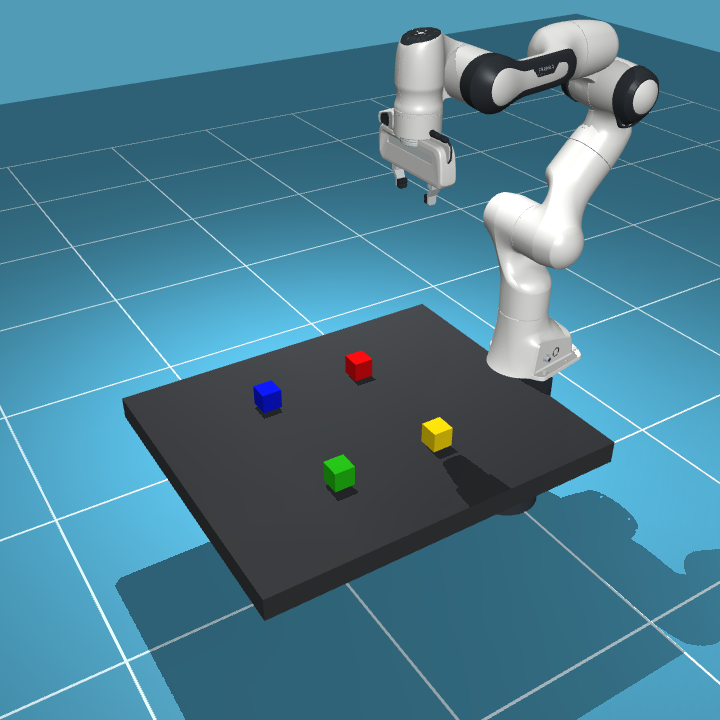
\includegraphics[width=\linewidth]{blocks_initial.png}\caption{Blocks：两组积木堆叠}\end{subfigure}\hfill
\begin{subfigure}{.31\linewidth}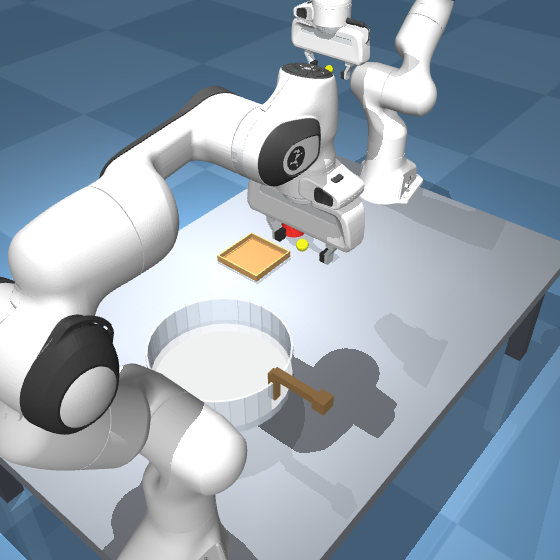
\includegraphics[width=\linewidth]{pour_initial.png}\caption{Pour：持盆接球}\end{subfigure}
\par\medskip
\begin{subfigure}{.39\linewidth}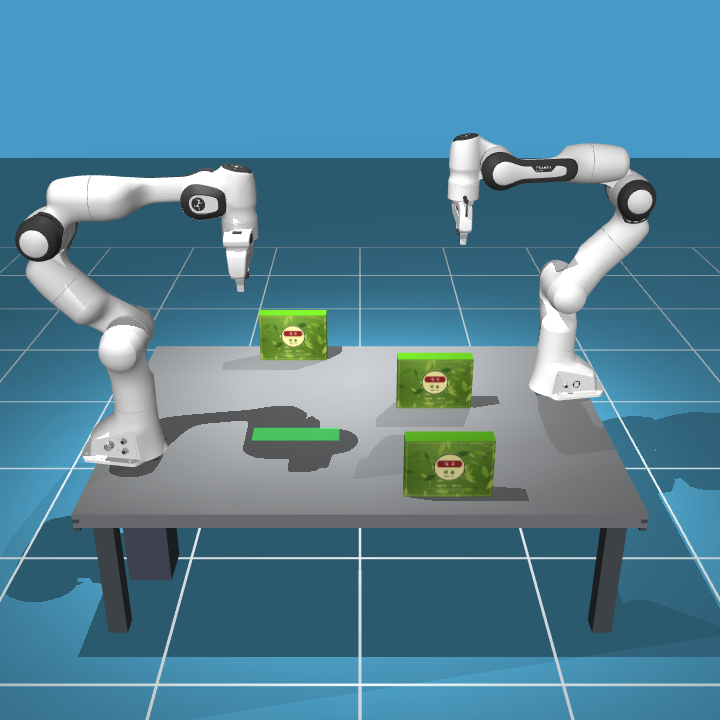
\includegraphics[width=\linewidth]{handover_initial.png}\caption{Handover：活动茶盒交接}\end{subfigure}\hspace{.05\linewidth}
\begin{subfigure}{.39\linewidth}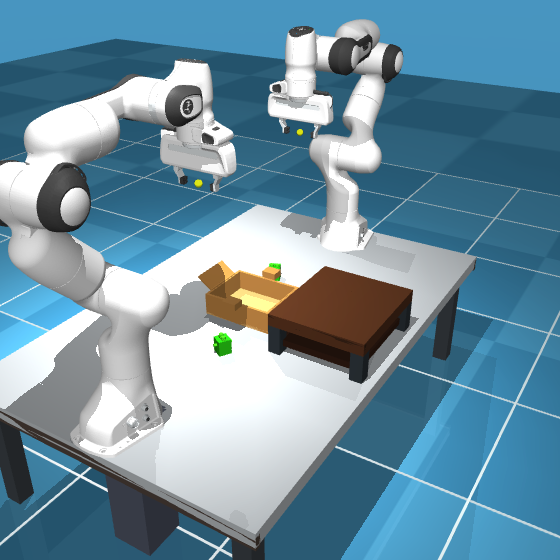
\includegraphics[width=\linewidth]{storage_initial.png}\caption{Storage：装箱与双臂上架}\end{subfigure}
\caption{五个冻结场景的真实仿真输入画面。物体外观包含便于辨识的视觉几何，控制与验收仍依赖各场景的物理碰撞几何。后三个场景使用明确披露的weld抓持辅助。}
\label{fig:scenes}
\end{figure}

\subsection{分层实验协议与数据选择}
实验分为四组，不能把它们相加为同一种成功率。
\begin{enumerate}
\item \textbf{模型与程序构造。}记录候选模型、程序输出、失败反馈和复用链。Cover采用约束下的模型schema提出；Blocks迁移已生成schema；双臂采用参考初始化及执行效果修订。
\item \textbf{冻结任务执行。}在工程迭代后选定的模型与程序上，运行9个声明目标对应的17次任务，检查113次动作转移与终态稳定窗口。这是条件性验收，不是未经选择的独立随机评测。
\item \textbf{同轨迹模型审计。}对每个双臂接地动作选择最终采样记录中最后一条已通过声明效果和物理条件的见证，共31条；在同一见证上比较原模型与修订模型的全状态匹配，不重新采样控制程序。
\item \textbf{统一相机诊断。}使用原接受程序和Oracle运动目标，进行5次相机兼容性运行；采集77组同步关键帧、282张图像。在其中7个场景--阶段--目标组合上，比较4个视角的28次实际Qwen输出。该组新图像不进入机器人控制。
\end{enumerate}

17次冻结执行中，Cover包括C1/C2/C3的基准及C3的两次$\pm2$\,mm扰动；Blocks包括三个目标各两种初态；Handover与Storage分别使用基准和一次小扰动初态，扰动幅度分别为$\pm2$\,mm与$\pm3$\,mm。Pour的布局扰动参数为零，第二次仅是重复运行。部分配置和提示曾在迭代中参考失败结果修改，因此本文统一称其为“冻结后复验与小扰动检查”，不把所有额外种子称为从未参与开发的盲测集。

\subsection{指标与对照的解释}
任务完成指标要求目标在终态及预设稳定窗口内成立，并满足场景特定的释放、姿态、支撑和历史事件条件。动作一致性计数为满足式\eqref{eq:full}的动作转移数。代码采样记录另外区分解析失败、接口失败、执行异常、声明效果缺失和未建模状态变化。三种双臂辅助控制的成功不与单臂无weld结果合并解释为同一物理条件下的性能。

视觉诊断统计模型是否返回合法二维点或拒答，并在语义目标可对应时比较参考投影。以真值高度代入式\eqref{eq:ray}得到的水平误差，仅表示“假设高度已知”时的条件误差，不是部署中的三维定位精度。几何投影往返误差是实现自洽性检查，也不能充当视觉模型准确率。

本文没有完成统一预算下的手写程序、无反馈语言模型、原CABTO、确定性效果修订器和完整改进流程之间的对照。因此，下文的流程前后比较属于诊断证据或同轨迹逻辑审计，不称为因果消融，也不报告统计显著性。由于任务异质、样本量小且程序经过选择，本文不以二项独立同分布假设为17/17计算可泛化置信区间。

\section{实验结果与分析}
\subsection{冻结任务执行与分层结果}
表\ref{tab:main}给出从原始JSON重新汇总的结果。五个场景共43个接地动作实例，覆盖9个声明目标。17次冻结执行均通过终态验收，113次动作转移均与最终符号模型匹配。其中，Cover和Blocks的11次任务、51次转移使用Qwen粗定位、RGB几何细化与高度先验；三个双臂场景的6次任务、62次转移使用Oracle几何和显式weld辅助。

\begin{table}[htbp]
\centering\small
\caption{最终冻结执行结果。所有分母仅指表中保留的复验回合；不包含构造阶段失败，因此不能作为模型从零构造系统的成功率。}
\label{tab:main}
\begin{tabularx}{\linewidth}{l c c c Y}
\toprule
场景 & 任务通过 & 转移匹配 & 动作步数 & 感知与抓持条件 \\
\midrule
Cover & 5/5 & 29/29 & 3、5、7 & Qwen＋RGB＋高度先验；无weld\\
Blocks & 6/6 & 22/22 & 3、3、5 & Qwen＋RGB＋高度先验；无weld\\
Pour & 2/2 & 20/20 & 10 & Oracle几何；weld辅助；零扰动重复\\
Handover & 2/2 & 14/14 & 7 & Oracle几何；盒面接触门控weld辅助\\
Storage & 2/2 & 28/28 & 14 & Oracle几何；双臂weld辅助搬箱\\
\midrule
合计 & 17/17 & 113/113 & 3--14 & 异质条件下的验收计数，不作统一性能排名\\
\bottomrule
\end{tabularx}
\end{table}

Cover全部已放置物体的最大水平目标误差为3.70\,mm，终态接触、释放和回HOME均通过；基准Blocks联合任务中，黄色和红色上层积木水平误差分别约1.98\,mm和3.08\,mm。双臂结果应结合辅助模式理解：Handover基准任务中盒体最终水平误差约0.52\,mm，但运输过程中使用了接触门控weld，因而该数值不能证明无辅助摩擦夹持的精度。Storage通过包含、货架支撑、姿态与释放检查，但没有新增覆盖全程的机器人接触历史审计；不能据此概括为五场景均经过同强度的无碰撞验证。

\begin{figure}[htbp]
\centering
\begin{subfigure}{.31\linewidth}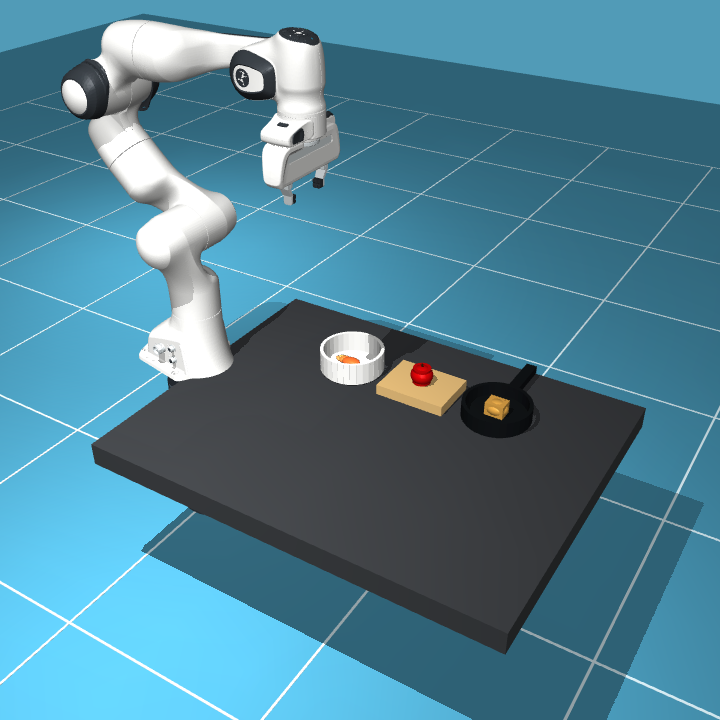
\includegraphics[width=\linewidth]{cover_final.png}\caption{Cover终态：三物体归位}\end{subfigure}\hfill
\begin{subfigure}{.31\linewidth}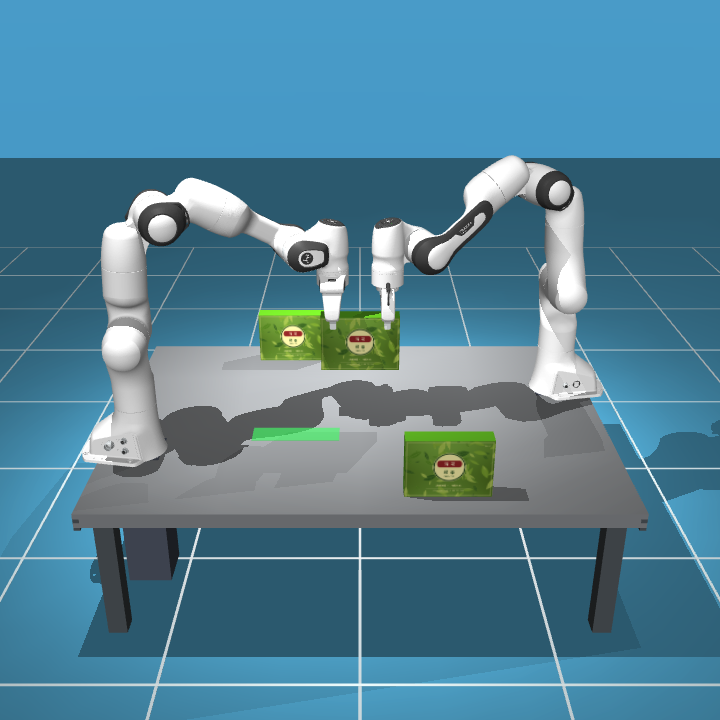
\includegraphics[width=\linewidth]{handover_dual_hold.png}\caption{交接中的双侧持有阶段}\end{subfigure}\hfill
\begin{subfigure}{.31\linewidth}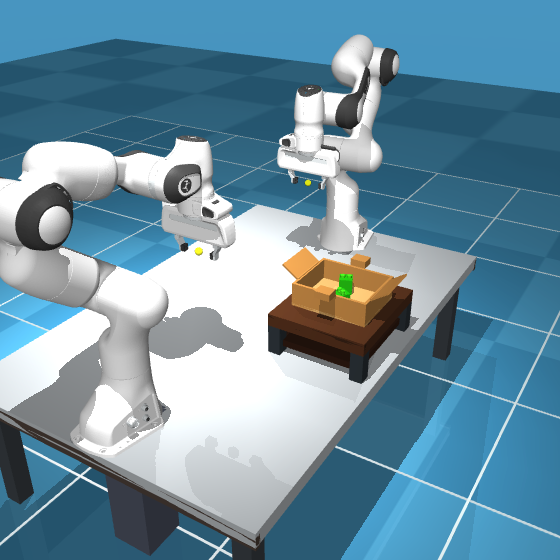
\includegraphics[width=\linewidth]{storage_final.png}\caption{纸箱获货架支撑并退手}\end{subfigure}
\caption{原始执行记录中的代表性状态。中、右图来自weld辅助的双臂分支，展示实际事件顺序与终态，不作为无辅助抓持的证据。}
\label{fig:rollouts}
\end{figure}

\subsection{全状态检查揭示了什么}
对31条双臂接地动作见证进行配对审计时，所有见证已经通过原声明效果检查，但只有21条与原动作模型的整个观测后继状态相等。其余10条并非都表现为物理失败，而是模型漏掉了执行后成立或消失的事实。表\ref{tab:witness}给出逐场景结果。

\begin{table}[htbp]
\centering\small
\caption{相同训练执行见证上的逻辑审计，以及修改后另行执行的完整任务复验。中间两列是同一轨迹的模型比较，不是两套控制策略的随机性能对照。}
\label{tab:witness}
\begin{tabularx}{\linewidth}{l c c c Y}
\toprule
场景 & 原模型全匹配 & 修订动作数 & 新模型同见证匹配 & 另行复验转移匹配 \\
\midrule
Pour & 8/10 & 2 & 10/10 & 20/20\\
Handover & 5/7 & 2 & 7/7 & 14/14\\
Storage & 8/14 & 6 & 14/14 & 28/28\\
\midrule
合计 & 21/31 & 10 & 31/31 & 62/62\\
\bottomrule
\end{tabularx}
\end{table}

三个例子说明遗漏效果的性质。第一，接收臂抓住茶盒后，原模型记录了双侧持有，却未显式增加接收臂持有谓词；局部任务可继续执行，但完整状态预测缺项。第二，交出臂释放后，原观测器中的交接位谓词因其依赖供方持有而失效，原模型没有删除它。第三，纸箱抬升会同时改变两臂持有状态与槽位空闲判据，即使两个物品仍在箱内，现有槽位判据的定义也会导致额外事实变化。具体而言，现有\code{slot_free(i)}使用随箱体变化的槽位水平坐标，却以固定桌高加底板厚度及物体半高为竖直参照，要求物体高度差小于20\,mm、水平各分量差小于两倍物体半尺寸加2\,mm才判为占用。\code{packed(i)}则将物体角点变换到箱体局部坐标系检查包含。箱体抬起后，前者可因固定高度参照失配而变为真，后者仍为真。因而这部分修订适配了当前观测器的语义局限，而不是发现了普适的“抬箱使槽位空闲”规律。后续应将占用高度统一到箱体局部系，并重新学习或验证相关效果；本文为避免追溯性改变实验含义，保留原观测器与原数据。

本研究没有通过删除观测字段使差异消失，而是将前后状态和差异交给模型，记录其实际补丁，再逐条核验并重规划。10处补丁在相同见证上全部满足完整等式；保持程序源码不变的新任务执行进一步得到62/62次双臂转移匹配。该结果支持全状态验收的诊断价值，但其“31/31”包含了对训练见证的适配，不应当作未见连续状态上的泛化准确率。

\subsection{生成能力与接口设计的共同影响}
早期小模型和9B非思考模式中均出现过错误契约、重复输出、截断及反馈回抄。较大的参数量没有自动消除这些问题。Cover中采用有界推理、单独最终JSON收束与符号检查后得到可用模型。低层采样中，聚焦局部动作语义有助于避免把完整任务写入一个Pick程序，但不同提示之间并非等预算、同状态的随机对照，因此只能作为调试现象而不是定量增益归因。

表\ref{tab:sampling}报告最终保存的采样／续跑链中保留的候选验证条目数。该数字包含成功链上的失败尝试与部分复用验证，但未覆盖所有被放弃的模型提出、提示探针、前置程序重放和人工迭代。尤其不能用“动作数除以验证条目数”定义模型生成成功率：复用没有新推理调用，同一程序也可能在不同对象上分别验证。

\begin{table}[htbp]
\centering\small
\caption{最终保存采样链的规模与来源。条目数是档案范围内的观测量，不是完整开发成本。}
\label{tab:sampling}
\begin{tabularx}{\linewidth}{l c c Y}
\toprule
场景 & 接受动作数 & 保留验证条目 & 主要来源与边界 \\
\midrule
Cover & 7 & 14 & 本地9B生成；土豆两动作复用已接受同类源码并重验\\
Blocks & 5 & 5 & Cover模型schema与程序原文迁移，不是五次新生成\\
Pour & 10 & 26 & 兼容历史模型程序复用；拆分返还接口后进行新采样\\
Handover & 7 & 19 & 本地模型采样与已有生成示例；空臂HOME按同类复用\\
Storage & 14 & 20 & 历史细粒度程序与新采样结合；显式撤离及跨对象重验\\
\bottomrule
\end{tabularx}
\end{table}

一些失败直接来源于接口与终止语义，而非抽象规划。Storage的旧放置程序没有竖直退手，旧停泊接口又隐含避障抬升。新接口将抬升单独暴露后，模型遗漏该调用会被运行时拒绝。Handover的接收程序曾缺少接近或闭爪，只有到达位姿并建立真实接触证据后才允许显式weld附着。Pour返还程序曾把目标支撑面参数误当高度标量，或将安全通道目标与放置目标混用；补充精确失败信息并保留最近一次源码后才完成新采样。这些例子表明，CABTO的有效工作单元应是“模型、程序、接口语义和验证器”的组合，而非孤立的文本推理。

\subsection{单臂视觉接地与几何误差}
Cover早期试验中，3B模型能够定位并抓起小虾，但持物后的碗定位出现约63\,mm的水平偏差，放置失败。基于粗点裁剪并放大的尝试仍出现约49\,mm双视角分歧，被既定25\,mm一致性门限拒绝。后续修复综合改变了观测角度、RGB细化、静态支撑物观测时机及对应特征高度，最终完成表\ref{tab:main}中的视觉任务。因此，不能把前后结果仅归因于裁剪、相机角度或单一提示词。

图\ref{fig:covervision}展示真实控制调用中的粗点与RGB细化。碗沿和锅沿是可见轮廓，放置目标却在内部支撑面上；先按照轮廓所在高度求水平位置，再使用相应支撑面定义放置高度，可以避免将这两个几何对象混同。在Blocks中，模型对支撑块的重复读取可能受到持物夹爪遮挡，因而在运动前观测位置保持受约束的支撑块，并对原图、细化结果及缓存读取分别记录。此类工程先验是当前可靠性的组成部分，不是无需模型和场景信息的开放世界定位。

\begin{figure}[htbp]
\centering
\begin{subfigure}{.46\linewidth}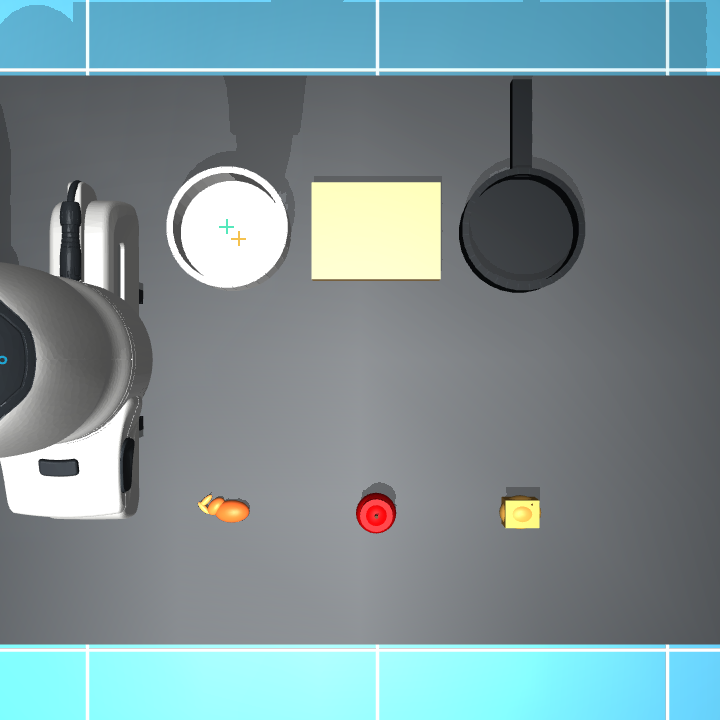
\includegraphics[width=\linewidth]{cover_bowl_overlay.png}\caption{碗区域：模型粗点与轮廓细化}\end{subfigure}\hfill
\begin{subfigure}{.46\linewidth}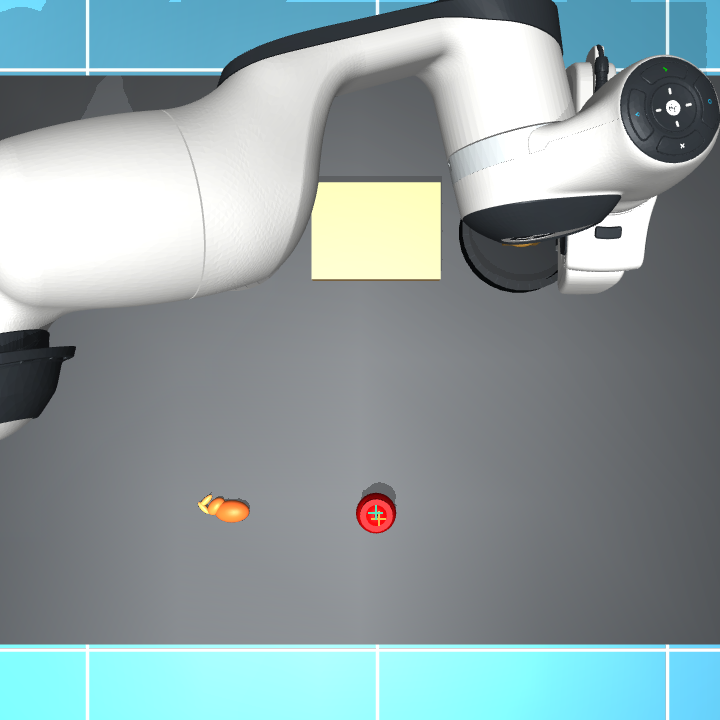
\includegraphics[width=\linewidth]{cover_apple_overlay.png}\caption{苹果区域：模型粗点与几何细化}\end{subfigure}
\caption{Cover实际视觉控制调用中的图像。黄色十字为模型粗点，绿色十字为RGB细化点；绿色不是仿真真值。物体高度和几何类别先验仍由冻结场景提供。}
\label{fig:covervision}
\end{figure}

\subsection{统一相机提高了可检查性，但尚未建立双臂视觉控制}
在统一相机试验中，五个场景全部保留原物理数组，增加相机节点后原接受程序均能完成任务。记录得到77组同步关键帧和282张图像；每组多相机图像采集之间不推进仿真。相机世界外参随手部实际运动，测得的局部安装关系保持不变。最大投影--平面往返误差约$1.01\times10^{-15}$\,m，只表明几何代码在浮点精度下自洽，不能解释为真实视觉定位达到了该精度。

图\ref{fig:cameras}给出相机实际成像。腕部近景能够放大积木和盒侧面，但持物自身也会进入前景；全局俯视可获得布局，却可能同时被机械臂遮住关键区域。因此，统一安装参数和统一相机接口是复现实验的基础，而不是所有任务阶段都具有良好可观测性的证明。

\begin{figure}[htbp]
\centering
\begin{subfigure}{.31\linewidth}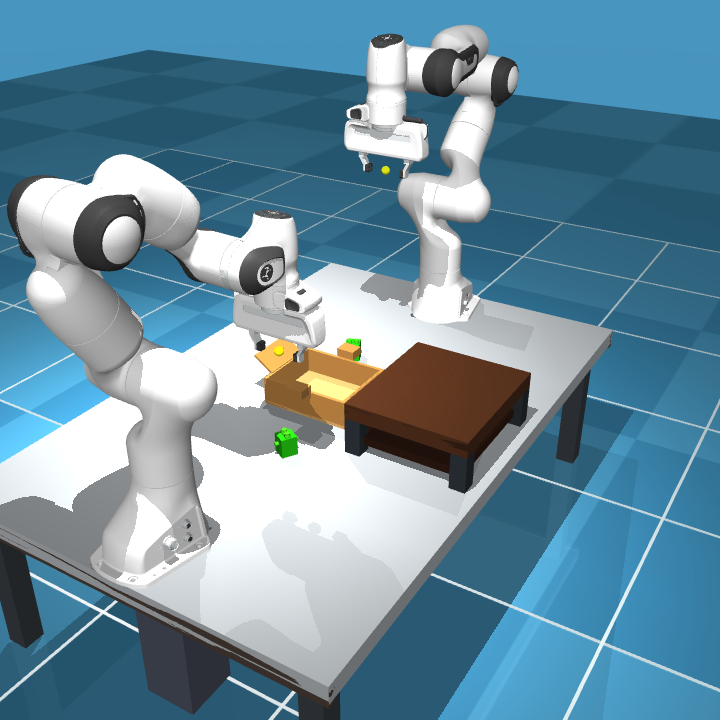
\includegraphics[width=\linewidth]{storage_old_item.png}\caption{Storage原全景}\end{subfigure}\hfill
\begin{subfigure}{.31\linewidth}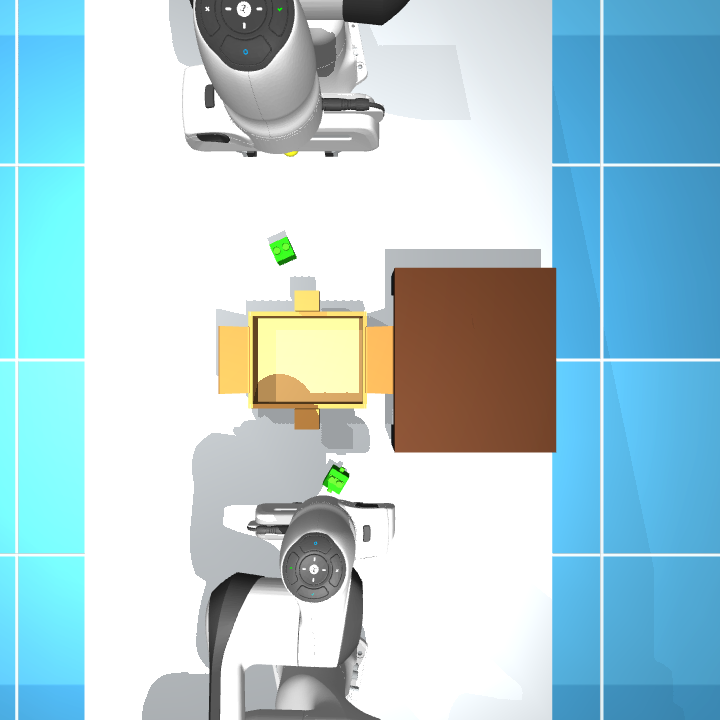
\includegraphics[width=\linewidth]{storage_global_item.png}\caption{同帧全局俯视}\end{subfigure}\hfill
\begin{subfigure}{.31\linewidth}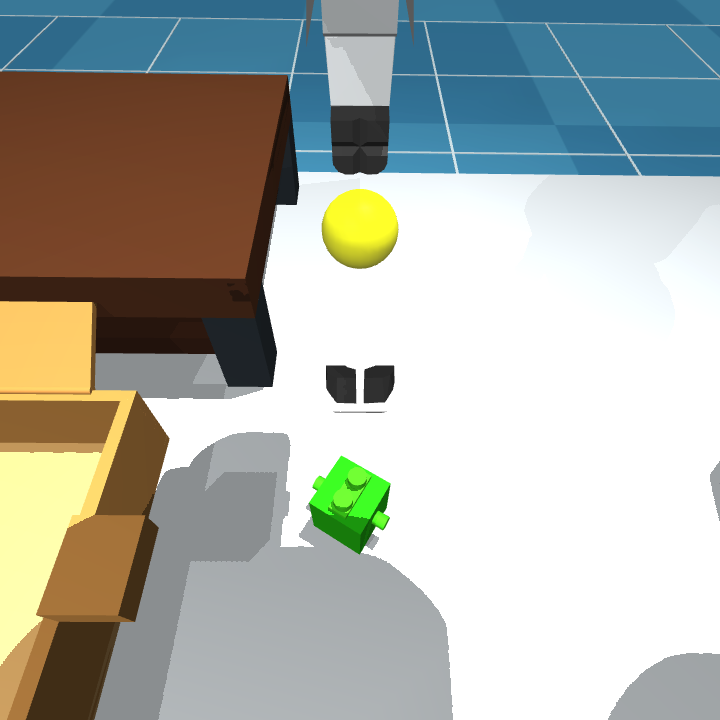
\includegraphics[width=\linewidth]{storage_wrist_item.png}\caption{同帧右腕近景}\end{subfigure}
\par\medskip
\begin{subfigure}{.31\linewidth}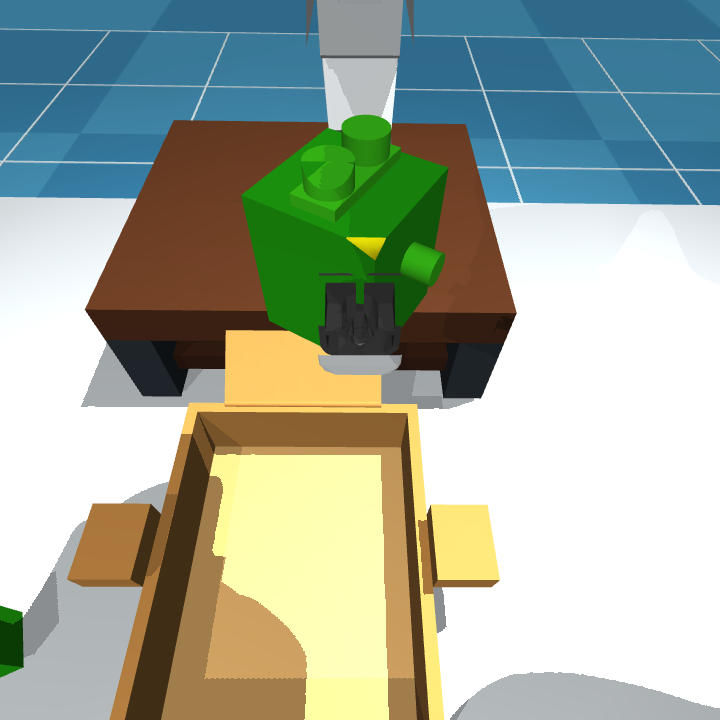
\includegraphics[width=\linewidth]{storage_wrist_slot.png}\caption{持物后腕部观察箱内}\end{subfigure}\hfill
\begin{subfigure}{.31\linewidth}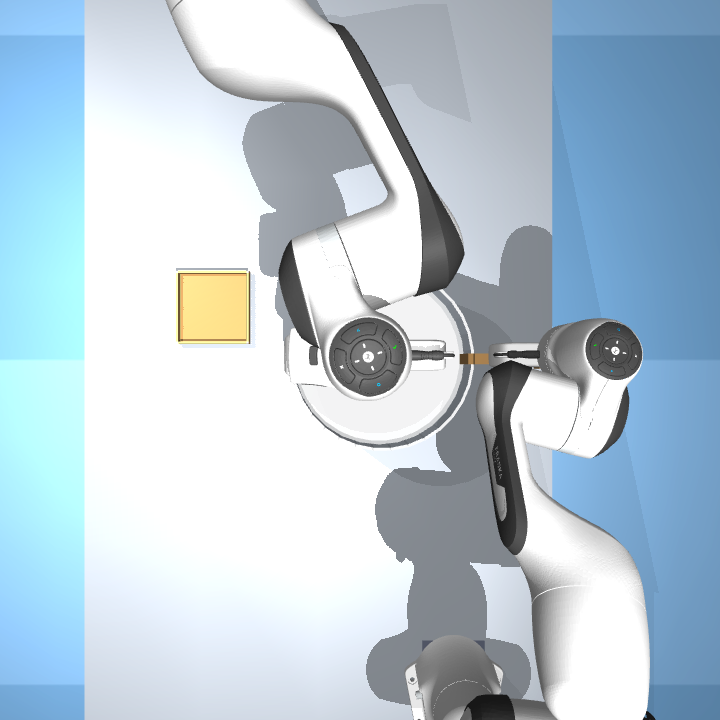
\includegraphics[width=\linewidth]{pour_global.png}\caption{Pour全局视角仍有遮挡}\end{subfigure}\hfill
\begin{subfigure}{.31\linewidth}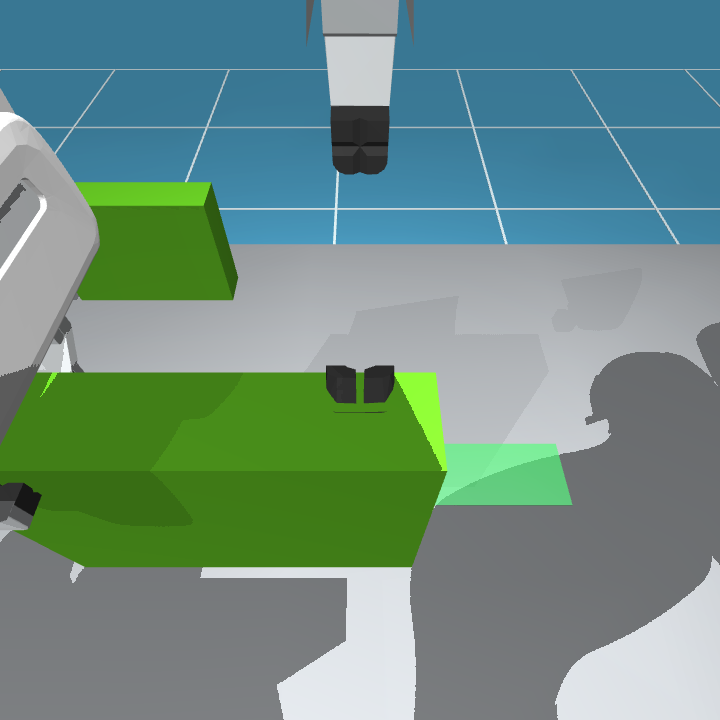
\includegraphics[width=\linewidth]{handover_wrist.png}\caption{Handover接收阶段腕部图}\end{subfigure}
\caption{统一相机配置的真实成像。上排为同一Storage物理状态；下排为不同任务阶段的示例。相机兼容性运行仍使用Oracle目标，不将这些新图像追记为此前成功控制的输入。}
\label{fig:cameras}
\end{figure}

28次同帧、同提示对照中，18次返回点，10次拒答，分场景统计见表\ref{tab:camera}。Storage的16次均输出坐标，但其中存在同色物体身份混淆；Pour的8次只有2次返回点；Handover针对指定接持区的4个视角均拒答。输出率不是正确率，拒答也不单独证明目标不可见。由于部分提示要求的可见表面与评估参考的body原点或TCP目标并不相同，本文不将全部像素误差平均为一个“定位准确率”。

\begin{table}[htbp]
\centering\small
\caption{统一相机下的新Qwen诊断调用。所有调用均未驱动机器人；这不是抓取或放置成功率。}
\label{tab:camera}
\begin{tabularx}{\linewidth}{l c c c Y}
\toprule
场景 & 调用数 & 返回点 & 拒答 & 尚未排除的问题 \\
\midrule
Storage & 16 & 16 & 0 & 同色物体误认，箱内无标记槽位，持物遮挡\\
Pour & 8 & 2 & 6 & 把手与夹爪重叠，源臂遮挡盆内，目标高度语义\\
Handover & 4 & 0 & 4 & 指定盒面接持区辨认，双臂近距离遮挡\\
\midrule
合计 & 28 & 18 & 10 & 可解析二维点与可执行位姿之间仍有未闭合环节\\
\bottomrule
\end{tabularx}
\end{table}

这里包含一项对方法适用性具有约束作用的负面结果：即使相机位置已经统一并通过几何自洽检查，视觉语言模型也不一定能够稳定提供符合当前动作语义的点。对Storage，应先识别箱体与物体身份，再由箱体姿态及声明槽位偏移获得目标；对Pour和Handover，还需要选择不被当前持物姿态遮挡的观测时机，并验证接触部位。当前系统没有把诊断点强制输入控制，也没有使用真值选择误差较小的视角来制造闭环成功。

\section{讨论：方法价值与适用边界}
\subsection{方法价值与当前最强证据}
本研究认为，CABTO最有价值的部分是把语言模型从直接决定任务成功的执行者，转变为能够接受规划与物理反驳的候选生成器。其高层模型、低层程序和跨层反馈划分，使错误可以定位到不同对象：不可规划可能来自动作库覆盖不足；程序异常可能来自接口误用；局部目标达成但状态预测不符则可能来自遗漏效果。三个层次不应互相替代。

在现有数据中，最有解释力的证据并不是17/17这个汇总数字，而是31条原本通过声明效果检查的双臂见证中，有10条在全状态审计下暴露模型差异；这些差异由明确补丁解释后，同一源码在新回合中仍可实现完整任务。这为“执行反馈能够校正模型语义”提供了具体支持。同时，腕部与全局相机的负面诊断说明，规划和程序层面的进展并未自动解决视觉接地问题，系统的能力仍受未闭合环节约束。

\subsection{不能由当前结果推出的结论}
首先，语言模型作用尚未与工程先验充分分离。动作签名、谓词定义、控制接口、几何先验和提示编排仍有人工投入，三个双臂动作库又从参考模型初始化。局部代码序列生成和效果补丁生成有效，不意味着机器人能够自行发现任务所需的全部抽象。其次，有限策略失败不能证明模型前提不足，更不能作为不可实现性的判据。当前流程能处理一类遗漏效果，而前提的几何充分性、条件效果以及新谓词学习均未解决。

再次，完整观测状态一致性取决于观测器是否合适。若谓词定义错误，模型可能只是忠实拟合错误抽象；若监测器没有覆盖全程碰撞，则状态等式匹配仍可能漏掉安全问题。符号词表应在验收前冻结，监测器与程序权限应隔离，并通过独立几何或接触信号交叉检查。对于有历史依赖的事件，必须明确其来自执行监测状态，而不能将任意程序可写布尔变量当作物理事实。

最后，当前结果全部来自仿真。weld辅助改变了抓持动力学，理想腕部相机没有外壳与电缆，RGB分割依赖场景颜色和外观，且没有域随机化、真实传感器噪声与实机校准误差。即使一个仿真控制轨迹具有正确事件顺序，它仍不能替代实体机器人上的接触抓持验证。

\subsection{进一步研究的必要对照}
建立更强的比较性结论，需要在后续研究中完成以下对照。
\begin{enumerate}
\item 在相同场景、模型版本与候选预算下，比较无反馈程序生成、仅程序反馈、确定性效果差分修订和模型效果修订。报告生成调用、token、前置轨迹重放、运行时间与人工干预，而不仅报告最终任务完成。
\item 将布局、物体几何、摩擦和初始姿态划分为开发集与预先封存的测试集；对同一程序进行真正不回馈搜索的测试，检验动作前提覆盖边界。
\item 分离无weld与weld辅助结果，在双臂中逐步替换Oracle几何，比较固定全局、单腕与多视角定位，且所有比较使用同一语义目标与独立精度判据。
\item 增加受控扰动与故障注入，检验行为树反应性、失败后的重新规划以及已达目标是否被后续动作破坏。当前无扰动执行不能直接支持鲁棒性提升结论。
\end{enumerate}

这些对照将分别检验反馈是否有效、语言模型是否必要、控制辅助带来何种影响以及观察抽象能否跨分布成立。当前结果能够支持具体反例上的模型修订和固定任务集的可执行性，尚不足以回答人工成本降低幅度、相对于规则修订的优势或开放任务泛化能力。

\section{结论}
本文基于CABTO的行为树接地思想，构建了执行证据驱动的动作模型、细粒度程序及感知诊断验证流程。通过区分声明任务集上的符号完备性、全观测状态上的经验一致性与连续物理可执行性，系统能够识别局部效果检查忽略的状态变化，并在固定程序源码的条件下验证模型修订。五类仿真场景的17次冻结任务和113次动作转移通过验收，十处双臂遗漏效果获得实际模型补丁与后续执行支持。与此同时，双臂Oracle定位、weld辅助、人工接口先验和新视角打点失败明确限制了结论范围。当前证据支持CABTO作为可检查的神经符号系统构造框架；进一步研究应围绕前提充分性、感知与接触闭环、成本归因及预注册泛化评测展开，而不应将有限成功轨迹提升为普遍可靠性保证。

\section*{数据、代码与复现说明}
本文数值来自同一项目内已经保存的JSON、源码、图片与视频记录，未为本文补写任务成功结果。随稿提供\code{evidence.json}、\code{source_manifest.json}和\code{collect_evidence.py}，分别对应表格数据、原文件SHA-256与只读数据抽取脚本。该脚本不启动模型推理或机器人仿真。LaTeX工程可独立编译；若要重新执行机器人任务，需要原\code{edps_cabto_exp}工程及其环境。作者贡献、基金、利益冲突与公开数据许可需由实际作者在投稿前确认，本稿不代为作出声明。

\printbibliography[heading=bibintoc,title={参考文献}]

\appendix
\begingroup\small\linespread{1.0}\selectfont
\ctexset{section={format=\large\bfseries},subsection={format=\normalsize\bfseries}}
\section{原始证据与计数口径}
\subsection{可追溯的实验目录}
表\ref{tab:paths}中的路径均相对于\code{edps_cabto_exp/outputs}。论文使用数据抽取时记录的文件哈希，而不以汇报网页中的文字作为唯一证据。Cover的最终程序来源与此前会话候选严格区分；双臂修订后的策略文件标记为待重验，是否通过以独立最终执行结果为准。

\begin{table}[htbp]
\centering\footnotesize
\caption{主要数据源及其证据用途。}\label{tab:paths}
\begin{tabularx}{\linewidth}{p{29mm}Y}
\toprule
证据组 & 相对路径与内容 \\
\midrule
Cover模型与代码 & \path{cover_cabto_fix/proposal_final_v2/models.json}；\path{cover_cabto_fix/sampling_9b_complete/policies.json}。\\
Cover冻结执行 & \path{cover_cabto_fix/final_visual/result.json}；\path{final_holdout1/result.json}与\path{final_holdout2/result.json}位于同一上级目录。\\
其余四场景执行 & \path{remaining_cabto/<task>/final_seed0/result.json}与\path{final_seed1/result.json}，其中\code{<task>}为blocks、pour、handover或storage。\\
双臂训练见证 & Pour使用\path{sampling_v5/policies.json}；Handover使用\path{sampling_v3/policies.json}；Storage使用\path{sampling_v2/policies.json}。均位于对应任务目录。\\
模型效果补丁 & \path{remaining_cabto/<task>/refinement/patch*.json}及\path{models.json}，保存真实模型回答、差异和前后状态。\\
统一相机运行 & \path{unified_cameras/selected_v3/<task>/result.json}及\path{frames/}，包括同帧RGB、动态标定、物理参数对比。\\
相机打点诊断 & \path{unified_cameras/pointing_v3/results.json}，28次新调用，不属于原任务控制输入。\\
\bottomrule
\end{tabularx}
\end{table}

计数中“9个目标”指五场景各自的目标规格，数量为$3+3+1+1+1$；“43个动作”指场景内接地实例之和$7+5+10+7+14$，包含schema复用，不是43次独立技能学习；“17次执行”包括重复与小扰动检查，不等于17个独立任务类别；“113次转移”是这些执行回合中的动作数，不包括候选搜索失败。独立相机兼容性运行的5次任务和28次打点诊断均未加入表\ref{tab:main}分母。

\subsection{十处实际效果修订}
下表保留模型补丁中的命题语义，缩写仅用于排版：$H_i$表示\code{holding(i,tray)}，$R_i$表示\code{hands_safe_for_lateral(i)}，$U$表示\code{hands_raised()}。所有补丁的原始完整字符串保存在\code{evidence.json}中。没有列入补丁的前提和控制源码在该修订阶段保持不变。

\begingroup\small
\setlength{\tabcolsep}{4pt}
\begin{longtable}{p{25mm}p{35mm}p{47mm}p{43mm}}
\caption{由真实执行差异触发的十处模型效果补丁。}\label{tab:patches}\\
\toprule 场景 & 动作 & 补充增加效果 & 补充删除效果\\\midrule
\endfirsthead
\toprule 场景 & 动作 & 补充增加效果 & 补充删除效果\\\midrule
\endhead
Pour & 源杯返还 & \code{parked(0)} & 无\\
Pour & 接收盆返还 & \code{at_source(basin)}；\code{parked(1)} & \code{receiver_separated()}\\
Handover & 接收臂抓盒面 & \code{receiver_holding(baton)} & 无\\
Handover & 供方释放并撤离 & 无 & \code{at_handover_pose(baton)}\\
Storage & 右臂抓物 & 无 & $U$、$R_1$\\
Storage & 右臂放物入箱 & $U$、$R_1$ & 无\\
Storage & 左臂抓物 & 无 & $U$、$R_0$\\
Storage & 左臂放物入箱 & $U$、$R_0$ & 无\\
Storage & 双臂抬箱 & $H_0$、$H_1$；\code{slot_free(0)}；\code{slot_free(1)} & 无\\
Storage & 货架上释放箱体 & 无 & $H_0$、$H_1$\\
\bottomrule
\end{longtable}
\endgroup

\subsection{软件验证与不能替代的物理验证}
统一相机模块新增27项测试，加上已有36项四场景接口测试、25项视觉测试、8项坐标来源测试、44项Cover方法测试和164项基础回归，共304项测试通过。这些测试检查接口边界、坐标约定、模型可达性、参数来源与不变性，不是304次机器人任务执行，更不能替代实机实验。相机几何往返误差接近机器精度同样只属于软件实现验证。

复用该证据集时，应同时保留失败目录、模型初始化来源、辅助开关和相机诊断标记。新增实验应形成新的冻结结果及分母，不将事后图像推理加入此前控制成功次数，也不以调整谓词词表或混用辅助条件的方式提高一致性计数。
\endgroup
\end{document}
